\documentclass{beamer}
\beamerdefaultoverlayspecification{<+->}
%
% Choose how your presentation looks.
%
% For more themes, color themes and font themes, see:
% http://deic.uab.es/~iblanes/beamer_gallery/index_by_theme.html
%
\mode<presentation>
{
  \usetheme{default}      % or try Darmstadt, Madrid, Warsaw, ...
  \usecolortheme{default} % or try albatross, beaver, crane, ...
  \usefonttheme{default}  % or try serif, structurebold, ...
  \setbeamertemplate{navigation symbols}{}
  \setbeamertemplate{caption}[numbered]
} 

\usepackage[english]{babel}
\usepackage[utf8]{inputenc}
\usepackage[T1]{fontenc}
\usepackage{hyperref}
\usepackage{pgfplots}
\pgfplotsset{compat=1.7}

\hypersetup{
    colorlinks=true,
    linkcolor=blue,
    filecolor=magenta,      
    urlcolor=cyan,
    bookmarks=true,
    pdfpagemode=FullScreen,
    }

\title{Econ 200 Section AJ}
\author{Lukas Hager \\ \href{mailto:lghhager@uw.edu}{lghhager@uw.edu}}
\institute{Office Hours: Monday 8-9, Thursday 3:30-4:30}
\date{January 8, 2021}

\begin{document}

\begin{frame}
  \titlepage
\end{frame}

% Uncomment these lines for an automatically generated outline.
%\begin{frame}{Outline}
%  \tableofcontents
%\end{frame}

\section{Introduction}

\begin{frame}{Introduction}

\begin{itemize}
  \item Name
  \item Where you're from
  \item Are you physically at UW?
  \item Year in school
  \item If you know what you want to do, your major/planned major (undecided is totally cool too!)
\end{itemize}

\end{frame}

\begin{frame}{Introduction}

\begin{itemize}
  \item I'm a first year Ph.D. student at UW.
  \item I try to be really responsive via email, so don't hesitate to reach out.
  \item TA sessions will take place over Zoom
  \begin{itemize}
      \item Feel free to make suggestions about things that we can do differently! You likely have more experience with Zoom classes than I do, so your expertise and experience are valued.
      \item My personal preference is for you to keep your video on, if at all possible. I'd love to try to get to know you, and that connection will be easier if we can see each other!
  \end{itemize}
\end{itemize}

\end{frame}

\section{Student Responsibilities}

\begin{frame}{Student Responsibilities}
    \begin{itemize}
        \item Read the syllabus carefully!
        \item Do the readings for the lecture section \textit{before} the section.
        \item Write down answers to problems -- this is much better than doing them in your head.
        \item Your grade depends on the quality of your answers, not just getting the right answer.
        \item I \textit{highly} encourage you to form small groups to study and work with. Obviously this is tougher over Zoom, but it's highly beneficial.
    \end{itemize}
\end{frame}

\section{Your Questions}

\begin{frame}{Your Questions}
    Do you have questions about what you've read in the text or heard in lecture (or on the syllabus)?
\end{frame}

% \begin{frame}{Marginal Decisions}
%     Late in the semester, a friend tells you, “I was going to drop my psychology course so I could concentrate on doing well in my other courses, but I had already put so much time into the course that I decided not to drop it.”
%     \begin{enumerate}
%         \item What do you think of your friend’s reasoning?
%         \item How should your friend have made that decision?
%         \item What questions should you ask to help your friend make the decision?
%     \end{enumerate}
% \end{frame}

\begin{frame}{Marginal Decisions}
    Late in the semester, a friend tells you, “I was going to drop my psychology course so I could concentrate on doing well in my other courses, but I had already put so much time into the course that I decided not to drop it.”
\end{frame}

\begin{frame}[t]{Marginal Decisions}
    Late in the semester, a friend tells you, “I was going to drop my psychology course so I could concentrate on doing well in my other courses, but I had already put so much time into the course that I decided not to drop it.”
    \begin{enumerate}
        \item[1.] What do you think of your friend’s reasoning?
    \end{enumerate}
\end{frame}

\begin{frame}[t]{Marginal Decisions}
    Late in the semester, a friend tells you, “I was going to drop my psychology course so I could concentrate on doing well in my other courses, but I had already put so much time into the course that I decided not to drop it.”
    \begin{enumerate}
        \item[2.] How should your friend have made that decision?
    \end{enumerate}
\end{frame}

\begin{frame}[t]{Marginal Decisions}
    Late in the semester, a friend tells you, “I was going to drop my psychology course so I could concentrate on doing well in my other courses, but I had already put so much time into the course that I decided not to drop it.”
    \begin{enumerate}
        \item[3.] What questions should you ask to help your friend make the decision?
    \end{enumerate}
\end{frame}

\begin{frame}{Scarcity and Tradeoffs}
    Consider and organization that exists to help the poor. The leaders of the organization are discussing alternative methods of helping the poor when one asserts, “If even one poor person is helped with this method, then all of our time and money would have been worth it.”
\end{frame}

\begin{frame}[t]{Scarcity and Tradeoffs}
    Consider and organization that exists to help the poor. The leaders of the organization are discussing alternative methods of helping the poor when one asserts, “If even one poor person is helped with this method, then all of our time and money would have been worth it.”
    \begin{enumerate}
        \item[1.] Do you agree? 
    \end{enumerate}
\end{frame}

\begin{frame}[t]{Scarcity and Tradeoffs}
    Consider and organization that exists to help the poor. The leaders of the organization are discussing alternative methods of helping the poor when one asserts, “If even one poor person is helped with this method, then all of our time and money would have been worth it.”
    \begin{enumerate}
        \item[2.] What other factors should you consider?
    \end{enumerate}
\end{frame}

\begin{frame}[t]{Scarcity and Tradeoffs}
    Consider and organization that exists to help the poor. The leaders of the organization are discussing alternative methods of helping the poor when one asserts, “If even one poor person is helped with this method, then all of our time and money would have been worth it.”
    \begin{enumerate}
        \item[3.] What if the person speaking is Bill Gates (the world’s richest person)? Are the considerations different?
    \end{enumerate}
\end{frame}

\begin{frame}{PPF/Comparative Advantage}
    The following table shows the tradeoffs you face in allocating time to study for your upcoming economics and chemistry exams:
    \begin{table}[]
    \begin{tabular}{l|l|l|l|l|}
    \cline{2-5}
                                 & \multicolumn{2}{l|}{Hours Spent Studying} & \multicolumn{2}{l|}{Exam Score} \\ \hline
    \multicolumn{1}{|l|}{Choice} & Economics           & Chemistry           & Economics      & Chemistry      \\ \hline
    \multicolumn{1}{|l|}{A}      & 5                   & 0                   & 95             & 70             \\ \hline
    \multicolumn{1}{|l|}{B}      & 4                   & 1                   & 93             & 78             \\ \hline
    \multicolumn{1}{|l|}{C}      & 3                   & 2                   & 90             & 84             \\ \hline
    \multicolumn{1}{|l|}{D}      & 2                   & 3                   & 86             & 88             \\ \hline
    \multicolumn{1}{|l|}{E}      & 1                   & 4                   & 81             & 90             \\ \hline
    \multicolumn{1}{|l|}{F}      & 0                   & 5                   & 75             & 91             \\ \hline
    \end{tabular}
    \end{table}
\end{frame}

\begin{frame}[t]{PPF/Comparative Advantage}
    Use the data in the table to draw a production possibility frontier graph with your Econ score on the vertical axis and your Chem score on the horizontal axis.
    \begin{tikzpicture}
    \begin{axis}[
        axis lines = left,
        xmin=70, xmax=100,
        ymin=70, ymax=100,
        xtick={70,75,80,85,90,95},
        ytick={70,75,80,85,90,95},
        xlabel = Chemistry Score,
        ylabel = Economics Score,
    ]
    \end{axis}
    \end{tikzpicture}
\end{frame}

\begin{frame}[t]{PPF/Comparative Advantage}
    Label the points corresponding to choices C and D. If you are at choice C, what is the opportunity cost of increasing your Chemistry score by 4 points?
    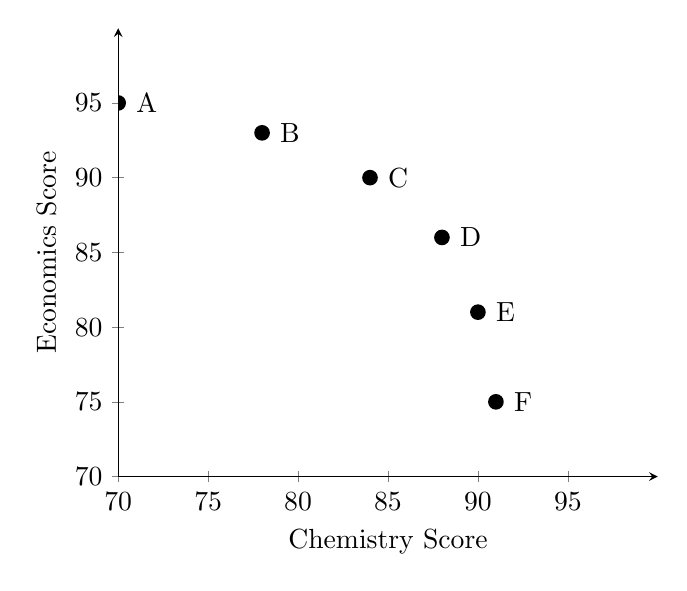
\begin{tikzpicture}
    \begin{axis}[
        axis lines = left,
        xmin=70, xmax=100,
        ymin=70, ymax=100,
        xtick={70,75,80,85,90,95},
        ytick={70,75,80,85,90,95},
        xlabel = Chemistry Score,
        ylabel = Economics Score,
    ]
    % \addplot[thick, mark=*, fill = black] coordinates {(70, 95)};
    % \addplot[thick, mark=*, fill = black] coordinates {(78, 93)};
    % \addplot[thick, mark=*, fill = black] coordinates {(84, 90)};
    % \addplot[thick, mark=*, fill = black] coordinates {(88, 86)};
    % \addplot[thick, mark=*, fill = black] coordinates {(90, 81)};
    % \addplot[thick, mark=*, fill = black] coordinates {(91, 75)};
    \node[label={0:{A}},circle,fill,inner sep=2pt] at (axis cs:70, 95) {};
    \node[label={0:{B}},circle,fill,inner sep=2pt] at (axis cs:78, 93) {};
    \node[label={0:{C}},circle,fill,inner sep=2pt] at (axis cs:84, 90) {};
    \node[label={0:{D}},circle,fill,inner sep=2pt] at (axis cs:88, 86) {};
    \node[label={0:{E}},circle,fill,inner sep=2pt] at (axis cs:90, 81) {};
    \node[label={0:{F}},circle,fill,inner sep=2pt] at (axis cs:91, 75) {};
    \end{axis}
    \end{tikzpicture}
\end{frame}

\begin{frame}{Tuna Spaghetti?}
    \begin{itemize}
        \item True/False/Uncertain: Mary purchases a tuna spaghetti at the school café for \$2 and just by smelling it she realizes that she doesn’t like it. The opportunity cost of throwing away the tuna spaghetti after purchasing it is \$2.
        \begin{itemize}
            \item False. Opportunity cost is about making a choice in the present. Obviously, since she does not have a choice over an action that has happened in the past, the \$2 she already spent is \textit{not} an opportunity cost.
        \end{itemize}
    \end{itemize}
\end{frame}

\begin{frame}{Tuna Spaghetti?}
    \begin{itemize}
        \item True/False/Uncertain: Consider the previous scenario. Mary could sell the untouched tuna spaghetti to her friend for \$1. The opportunity cost of throwing away the tuna spaghetti is still \$2.
        \begin{itemize}
            \item False. Opportunity cost is about making a choice in the present. If she throws away the tuna spaghetti she forgoes the \$1 she would have received for it. The opportunity cost here is \$1 which is what she can get for it now, not \$2 which is what she \textit{already} spent. 
        \end{itemize}
    \end{itemize}
\end{frame}

\beamerdefaultoverlayspecification{}
\begin{frame}{Tuna Spaghetti?}
    \begin{itemize}
        \item Consider the previous scenario. Mary purchases a tuna spaghetti at the school café for \$2 and just by smelling it she realizes that she doesn’t like it. Mary would like a hamburger instead of the tuna spaghetti, but decides that she will eat the tuna spaghetti she just purchased. A hamburger sells for \$2.50. She values a hamburger at \$4. The opportunity cost of eating the tuna spaghetti is then:
        \begin{enumerate}
            \item \$1.50
            \item \$2.50
            \item \$4.00
            \item \$6.50
        \end{enumerate}
    \end{itemize}
\end{frame}

\beamerdefaultoverlayspecification{<+->}
\begin{frame}{Tuna Spaghetti?}
    Option 1 is correct. If Mary decides to eat the tuna spaghetti she is forgoing the benefits of a hamburger which is \$4 foregone (a benefit not gained is a cost). She is avoiding the cost of hamburger, which is \$2.5  (a cost that is avoided is a benefit). Therefore, the opportunity cost of eating the tuna spaghetti is net benefit forgone: \[\$4 - \$2.50 = \$1.50\]
\end{frame}

% \begin{frame}{Review of Main Concepts}
% \begin{itemize}
%     \item Scarcity
%     \begin{itemize}
%         \item "Economics is the study of how scarce resources, that have alternative uses, are allocated amongst competing ends" (\textit{Principles of Microeconomics} p.13) 
%     \end{itemize}
%     \item Opportunity Cost
%     \begin{itemize}
%         \item "The cost of any activity is the highest-valued opportunity that is foregone when the activity is pursued" (\textit{Principles of Microeconomics} p.14) 
%     \end{itemize}
% \end{itemize}
% \end{frame}

% \section{Examples}

% \begin{frame}{Example 1}
%     \begin{itemize}
%         \item John has three choices for a vacation: seaside/beach, mountain cabin with hiking and, a fishing trip by the river (his least favorite choice). What is the opportunity cost in picking each of these vacations?
%         \begin{itemize}
%             \item The opportunity cost of choosing to go to the mountain cabin to hike is the beach vacation given up. The opportunity cost of the beach vacation is the mountain cabin given up. What about the fishing trip?
%         \end{itemize}
%     \end{itemize}
% \end{frame}

% \begin{frame}{Example 2}
%     \begin{itemize}
%         \item Jane decides to go to college instead of making money immediately by working full-time on a cruise ship after finishing high school.
%         \begin{itemize}
%             \item The opportunity cost of attending college full time includes forgoing a salaried job after high school. Also included in the opp. cost is the tuition, and cost of books and supplies for college could have been spent on other goods and services.
%         \end{itemize}
%     \end{itemize}
% \end{frame}

% \begin{frame}{Non-Example}
%     \begin{itemize}
%         \item Mona pays \$10 to go to a movie that lasts two hours and after 10 minutes she realizes that she really does not like the film. However, she continues to stay because she feels that she’s already spent ten dollars and wants to get her money’s worth. She continues to watch the film while thinking that she should have been spending time with her friends in the park and that is what she really wanted to do.
%         \begin{itemize}
%             \item She thinks the opportunity cost of walking out of the theatre after 10 minutes is the \$10 lost. She is wrong! The opportunity cost is missing the walk with her friends in the park
%         \end{itemize}
%     \end{itemize}
% \end{frame}

% \section{Questions}

% \begin{frame}{Question 1}
%     \begin{itemize}
%         \item True/False/Uncertain: Mary purchases a tuna spaghetti at the school café for \$2 and just by smelling it she realizes that she doesn’t like it. The opportunity cost of throwing away the tuna spaghetti after purchasing it is \$2.
%         \begin{itemize}
%             \item False. Opportunity cost is about making a choice in the present. Obviously, since she does not have a choice over an action that has happened in the past, the \$2 she already spent is \textit{not} an opportunity cost.
%         \end{itemize}
%     \end{itemize}
% \end{frame}

% \begin{frame}{Question 2}
%     \begin{itemize}
%         \item True/False/Uncertain: Consider the previous scenario. Mary could sell the untouched tuna spaghetti to her friend for \$1. The opportunity cost of throwing away the tuna spaghetti is still \$2.
%         \begin{itemize}
%             \item False. Opportunity cost is about making a choice in the present. If she throws away the tuna spaghetti she forgoes the \$1 she would have received for it. The opportunity cost here is \$1 which is what she can get for it now, not \$2 which is what she \textit{already} spent. 
%         \end{itemize}
%     \end{itemize}
% \end{frame}

% \beamerdefaultoverlayspecification{}
% \begin{frame}{Question 3}
%     \begin{itemize}
%         \item Consider the previous scenario. Mary purchases a tuna spaghetti at the school café for \$2 and just by smelling it she realizes that she doesn’t like it. Mary would like a hamburger instead of the tuna spaghetti, but decides that she will eat the tuna spaghetti she just purchased. A hamburger sells for \$2.50. She values a hamburger at \$4. The opportunity cost of eating the tuna spaghetti is then:
%         \begin{enumerate}
%             \item \$1.50
%             \item \$2.50
%             \item \$4.00
%             \item \$6.50
%         \end{enumerate}
%     \end{itemize}
% \end{frame}

% \beamerdefaultoverlayspecification{<+->}
% \begin{frame}{Question 3}
%     Option 1 is correct. If Mary decides to eat the tuna spaghetti she is forgoing the benefits of a hamburger which is \$4 foregone (a benefit not gained is a cost). She is avoiding the cost of hamburger, which is \$2.5  (a cost that is avoided is a benefit). Therefore, the opportunity cost of eating the tuna spaghetti is net benefit forgone: \[\$4 - \$2.50 = \$1.50\]
% \end{frame}

% \begin{frame}{Question 4}
%     \begin{itemize}
%         \item Jack is deciding between renting an apartment for one year and buying one. The monthly rent for the apartment is \$1,000 per month (\$12,000 per year). If he purchases the apartment, his mortgage would be the same (\$12,000) per year. Suppose that as a homeowner, he could subtract 10\% of his mortgage payment from his annual income tax payments. Considering no other costs to purchasing or renting the apartment and no change in the price of the apartment at the end of the year, what is Jack’s opportunity cost of renting the apartment for a year?
%         \begin{itemize}
%             \item At the end of the year, Jack will pay \$12,000 to rent the apartment, and will pay \$12,000 to buy it.
%             \item If he buys, he can remove a cost of \$1,200 to him at the end of the year by annual income taxes credits.
%             \item If he buys, he owns \$12,000 "worth" of apartment (equity), which he can sell and realize at the end of the year, if he wants to.
%             \item In sum, the opportunity cost is \[\$1200 + \$12000 = \$13200\]
%         \end{itemize}
%     \end{itemize}
% \end{frame}

% \begin{frame}{Question 5}
%     \begin{itemize}
%         \item What are the two sets of influences identified by the theory of consumer behavior?
%         \begin{itemize}
%             \item Constraints
%             \item Tastes
%         \end{itemize}
%         \item What are examples of each?
%         \item Which one of the two categories is essentially not measurable?
%         \item How can we develop the theory of consumer and explain consumer behavior if we are unable to measure tastes?
%         \begin{itemize}
%             \item We take tastes as given.
%         \end{itemize}
%     \end{itemize}
% \end{frame}
\end{document}
